% Options for packages loaded elsewhere
\PassOptionsToPackage{unicode}{hyperref}
\PassOptionsToPackage{hyphens}{url}
%
\documentclass[
]{article}
\usepackage{amsmath,amssymb}
\usepackage{lmodern}
\usepackage{iftex}
\ifPDFTeX
  \usepackage[T1]{fontenc}
  \usepackage[utf8]{inputenc}
  \usepackage{textcomp} % provide euro and other symbols
\else % if luatex or xetex
  \usepackage{unicode-math}
  \defaultfontfeatures{Scale=MatchLowercase}
  \defaultfontfeatures[\rmfamily]{Ligatures=TeX,Scale=1}
\fi
% Use upquote if available, for straight quotes in verbatim environments
\IfFileExists{upquote.sty}{\usepackage{upquote}}{}
\IfFileExists{microtype.sty}{% use microtype if available
  \usepackage[]{microtype}
  \UseMicrotypeSet[protrusion]{basicmath} % disable protrusion for tt fonts
}{}
\makeatletter
\@ifundefined{KOMAClassName}{% if non-KOMA class
  \IfFileExists{parskip.sty}{%
    \usepackage{parskip}
  }{% else
    \setlength{\parindent}{0pt}
    \setlength{\parskip}{6pt plus 2pt minus 1pt}}
}{% if KOMA class
  \KOMAoptions{parskip=half}}
\makeatother
\usepackage{xcolor}
\usepackage[margin=1in]{geometry}
\usepackage{longtable,booktabs,array}
\usepackage{calc} % for calculating minipage widths
% Correct order of tables after \paragraph or \subparagraph
\usepackage{etoolbox}
\makeatletter
\patchcmd\longtable{\par}{\if@noskipsec\mbox{}\fi\par}{}{}
\makeatother
% Allow footnotes in longtable head/foot
\IfFileExists{footnotehyper.sty}{\usepackage{footnotehyper}}{\usepackage{footnote}}
\makesavenoteenv{longtable}
\usepackage{graphicx}
\makeatletter
\def\maxwidth{\ifdim\Gin@nat@width>\linewidth\linewidth\else\Gin@nat@width\fi}
\def\maxheight{\ifdim\Gin@nat@height>\textheight\textheight\else\Gin@nat@height\fi}
\makeatother
% Scale images if necessary, so that they will not overflow the page
% margins by default, and it is still possible to overwrite the defaults
% using explicit options in \includegraphics[width, height, ...]{}
\setkeys{Gin}{width=\maxwidth,height=\maxheight,keepaspectratio}
% Set default figure placement to htbp
\makeatletter
\def\fps@figure{htbp}
\makeatother
\setlength{\emergencystretch}{3em} % prevent overfull lines
\providecommand{\tightlist}{%
  \setlength{\itemsep}{0pt}\setlength{\parskip}{0pt}}
\setcounter{secnumdepth}{5}
\newlength{\cslhangindent}
\setlength{\cslhangindent}{1.5em}
\newlength{\csllabelwidth}
\setlength{\csllabelwidth}{3em}
\newlength{\cslentryspacingunit} % times entry-spacing
\setlength{\cslentryspacingunit}{\parskip}
\newenvironment{CSLReferences}[2] % #1 hanging-ident, #2 entry spacing
 {% don't indent paragraphs
  \setlength{\parindent}{0pt}
  % turn on hanging indent if param 1 is 1
  \ifodd #1
  \let\oldpar\par
  \def\par{\hangindent=\cslhangindent\oldpar}
  \fi
  % set entry spacing
  \setlength{\parskip}{#2\cslentryspacingunit}
 }%
 {}
\usepackage{calc}
\newcommand{\CSLBlock}[1]{#1\hfill\break}
\newcommand{\CSLLeftMargin}[1]{\parbox[t]{\csllabelwidth}{#1}}
\newcommand{\CSLRightInline}[1]{\parbox[t]{\linewidth - \csllabelwidth}{#1}\break}
\newcommand{\CSLIndent}[1]{\hspace{\cslhangindent}#1}
\usepackage{amstext}
\usepackage{amsmath}
\usepackage{booktabs}
\usepackage{longtable}
\usepackage{array}
\usepackage{multirow}
\usepackage{wrapfig}
\usepackage{float}
\usepackage{colortbl}
\usepackage{pdflscape}
\usepackage{tabu}
\usepackage{threeparttable}
\usepackage{threeparttablex}
\usepackage[normalem]{ulem}
\usepackage{makecell}
\usepackage{xcolor}
\usepackage{algorithm,algorithmic}
\AtBeginEnvironment{CSLReferences}{\small}
\usepackage{tabularx}
\usepackage{booktabs}
\usepackage{longtable}
\usepackage{array}
\usepackage{multirow}
\usepackage{wrapfig}
\usepackage{float}
\usepackage{colortbl}
\usepackage{pdflscape}
\usepackage{tabu}
\usepackage{threeparttable}
\usepackage{threeparttablex}
\usepackage[normalem]{ulem}
\usepackage{makecell}
\usepackage{xcolor}
\ifLuaTeX
  \usepackage{selnolig}  % disable illegal ligatures
\fi
\IfFileExists{bookmark.sty}{\usepackage{bookmark}}{\usepackage{hyperref}}
\IfFileExists{xurl.sty}{\usepackage{xurl}}{} % add URL line breaks if available
\urlstyle{same} % disable monospaced font for URLs
\hypersetup{
  pdftitle={Directed topic extraction with side information for sustainability analysis},
  pdfauthor={Maria Osipenko},
  hidelinks,
  pdfcreator={LaTeX via pandoc}}

\title{Directed topic extraction with side information for sustainability analysis}
\author{Maria Osipenko}
\date{}

\begin{document}
\maketitle

\hypertarget{abstract}{%
\section*{Abstract}\label{abstract}}
\addcontentsline{toc}{section}{Abstract}

Topic analysis represents each document of a text corpus in a low-dimensional latent topic space. In some cases, the desired topic representation is subject to specific requirements or guidelines constituting side information. For instance, sustainability-aware investors might be interested in automatically assessing firm sustainability aspects from the textual content of its corporate reports, focusing on the established 17 UN sustainability goals. The main corpus here contains the corporate report texts, while the texts with the definitions of the 17 UN sustainability goals represent the side information.

Under the assumption that both text corpora share a common low-dimensional subspace, we propose to represent them in such a space via directed topic extraction by matrix co-factorization. Both the main and the side text corpora are first represented as term-context matrices, which are then jointly decomposed into word-topic and topic-context matrices. The word-topic matrix is common to both text corpora, whereas the topic-context matrices contain specific representations in the shared topic space. A nuisance parameter, which allows to shift the focus between the error minimization of individual factorization terms, controls the extent to which the side information is taken into account.

With our approach, documents from the main and the side corpora can be related to each other in the resulting latent topic space. That is, the corporate reports are represented in the same latent topic space as the descriptions of the 17 UN sustainability goals, enabling a structured automatic sustainability assessment of the textual reports' content. We provide an algorithm for such directed topic extraction and propose techniques for visualizing and interpreting the results.

\hypertarget{introduction}{%
\section{Introduction}\label{introduction}}

The market for sustainable investments is growing steadily. However, there are no uniform standards for comparing or quantifying the sustainability levels of firms. Although several agencies now provide environmental, social, and governance (ESG) ratings, Berg, Kölbel, and Rigobon (2022) point out the disagreement among these ratings across different rating agencies. In this situation, it seems difficult to overview the ESG development of potential investment firms and decide based on an investor's ESG value system.

At the same time, large companies communicate their ESG-related strategies and actions in their sustainability reporting in the form of:

\begin{itemize}
\tightlist
\item
  Corporate responsibility reports
\item
  Sustainability reports
\item
  Environmental action reports
\end{itemize}

or similar sustainability-related reports. The intention of such reporting is to increase the transparency and accountability of ESG-related company actions for stakeholders, as noted by Soh (2014).

The analysis of sustainability-related textual sources has captured the attention of numerous researchers. To incorporate the specifics of sustainability texts, authors mainly rely on hand-crafted concepts and keywords. For instance, Liew, Adhitya, and Srinivasan (2014) use word and phrase frequencies to extract common trends and their importance from sustainability reporting based on sustainability content trees. Using their five content categories and the associated keywords, Landrum and Ohsowski (2017) perform the content analysis of sustainability-related corporate reports based on the proportion of contained keywords.

Tsalis et al. (2020) propose to evaluate the level of alignment of sustainability-related reports with the established 17 UN Sustainable Development Goals (SDGs, \url{https://sdgs.un.org/goals}). The SDGs represent an intergovernmental set of 17 goals that broadly address modern environmental and social challenges, adopted in 2015 by the UN General Assembly. The goal is to structure the information from textual sustainability reports with respect to the SDGs in a way that enables a sound comparison of companies' contributions to solving those major challenges. Tsalis et al. (2020) use a scoring system based on disclosure topics from the Global Reporting Initiative. The authors create a catalog of disclosure topics with respect to the SDGs using their expertise and previous research and use a scoring system to manually assign a score for each report for each catalog item, which they then aggregate.

A common drawback of these works is the extensive use of human expertise in the analysis, which reduces the objectivity of the results on one hand and is time-consuming on the other.

Kang and Kim (2022) propose to assess textual information in sustainability-related reports using SDGs as an anchor fully automatically. They choose a sentence similarity method to assess the relatedness of the reports to the goals. The approach of Kang and Kim (2022) is computationally intensive because each sentence in a report has to be compared to each sentence of an SDG text, and it does not provide a transparent report representation with low complexity, such as a representation in a low-dimensional topic space. The authors explain that they reject the classical word frequency-based topic analysis used in previous research because it cannot incorporate any ``predefined theme structure.'' In this paper, we overcome these limitations by proposing a topic analysis method using co-matrix factorization, which integrates any predefined structure into the analysis. Our method leverages the information in textual sources on sustainability via automatic topic extraction while considering the value system established by the 17 SDGs, thus providing a low-dimensional topic representation convenient for assessing the level of association between the SDGs and sustainability-related reports.

As a commonly used technique for structuring text data, topic analysis (Churchill and Singh (2022)) represents each document in a collection of documents in a low-dimensional latent topic space. The most popular classical methods are Latent (probabilistic) semantic analysis (Deerwester et al. (1990), Hofmann (1999)), Latent Dirichlet Allocation (LDA, Blei, Ng, and Jordan (2003)), as well as general-purpose dimension reduction methods like non-negative matrix factorization (NMF, Lee and Seung (2000), Vangara et al. (2020)), and extensions of these methods (e.g.~in Yang and Li (2015/07), Suleman and Korkontzelos (2021), and Figuera and García Bringas (2024)). Recently, deep neural network-based models have also been proposed (Zhao et al. (2021)).

Topic extraction for structuring text data has been extensively used in financial literature. For instance, Li et al. (2017) employs Latent Dirichlet Allocation (LDA) to structure financial stability reports. Yu Chen et al. (2017) compares Principal Component Analysis, NMF, LDA, and deep learning models for text analytics in banking. Amini, Bienstock, and Narcum (2018) perform automatic topic extraction using common methods specifically for sustainability-related reports. W. Chen et al. (2023) use LDA and neural network-based models to analyze news impact on financial markets. For a comprehensive review of text mining and topic analysis in finance literature, we refer to Loughran and McDonald (2016) and Gupta et al. (2020). Despite the popularity of LDA, Yong Chen et al. (2019) and Egger and Yu (2022) argue that NMF can outperform LDA by extracting interpretable topics, especially for short texts. Since we are going to cut the reports into small pieces of context, NMF is a promising technique for our needs. Moreover, Nugumanova et al. (2022) highlight the advantage of NMF-based methods for the efficient extraction of domain-specific terms, which is also relevant for our task with a sustainability focus.

Recently, several LDA-based topic extraction methods that allow for explicitly embedding known structures or side information have been proposed. For instance, Harandizadeh, Priniski, and Morstatter (2022) propose using word2vec embeddings combined with LDA and vocabulary priors to obtain interpretable word embeddings. Eshima, Imai, and Sasaki (n.d.) embed prespecified keywords in LDA for the same reason. Similarly, Watanabe and Zhou (2022) use seeded LDA with a carefully chosen seeded vocabulary to assist in classifying documents into specific categories. These approaches account for additional information in topic extraction. However, the drawback of the mentioned approaches in Watanabe and Zhou (2022) and Eshima, Imai, and Sasaki (n.d.) lies in the need for manual intervention for keyword or vocabulary specification. Harandizadeh, Priniski, and Morstatter (2022) use word vectors from a pretrained general-purpose word2vec model, so it is unclear whether their model works for specific domains such as sustainability reports.

On the other hand, some matrix factorization-based approaches integrate side information into dimension reduction. Rao et al. (2015) and later Zhang et al. (2020) propose integrating side information using graphs. They derive a graph-regularized version of matrix factorization and an associated alternating algorithm. However, their side information is not high-dimensional and incorporates few individual characteristics which form the basis for the graph links. Another way to consider high-dimensional additional information is through matrix co-factorization techniques. Co-factorization techniques factorize two or three matrices with some common cofactors simultaneously. For instance, Fang and Si (2011) consider user community information, and Luo et al. (2019) incorporate tagging and timestamps of ratings in their personalized recommendations via matrix co-factorization. This approach is transparent and easily adjustable. By introducing a nuisance parameter, which allows shifting focus between error minimization of individual factorization terms, additional flexibility is ensured.

In this paper, we propose a topic model based on non-negative matrix co-factorization (NMCF) to extract sustainability-related topics from related textual sources using the 17 UN goals as side information. The advantages of our approach include fully automated topic extraction (without manual keyword search), interpretability, adaptivity (via nuisance parameter \(\lambda\)), and a simple, scalable implementation.

The paper is structured as follows. In the next chapter, we explain the method used and derive the NMCF algorithm for topic extraction with side information. We also introduce the data in the form of sustainability-related reporting and the 17 UN goals and describe our preprocessing steps. The results of the application of our algorithm to the data follow. Finally, we conclude and discuss future research directions.

\hypertarget{data-and-methods}{%
\section{Data and Methods}\label{data-and-methods}}

In this section, we introduce our data basis and describe the preprocessing steps. Subsequently, we present our method of non-negative matrix co-factorization (NMCF) and derive the NMCF algorithm for topic extraction with side information.

\hypertarget{data-and-preprocessing}{%
\subsection{Data and preprocessing}\label{data-and-preprocessing}}

Large listed companies disclose their sustainability-related actions in corporate responsibility reports, sustainability reports, or similar releases on a regular basis. These reports aim to increase transparency and raise sustainability awareness within the companies. A typical report contains many pages with concise messages about sustainability actions and related pictures.

We use corporate responsibility and sustainability reports from the top eight listed tech companies with tickers: AAPL, AMZN, DELL, GOOG, IBM, INTC, MSFT, and SSU. The associated time period includes the years 2013 (or later) to 2022, depending on availability. The entities in the resulting main text corpus are the pages of the reports.

Our side information consists of the texts of the 17 UN SDGs, which we obtain from the UN website (\url{https://sdgs.un.org/goals}). The entities in the side information text corpus are the texts of the individual goals' descriptions.

All calculations are done in R (R Core Team (2023)). For the preprocessing on word level, we use R-Package Quanteda (Benoit et al. (2018)) to set up a corpus, to split in tokens, and compute the relative frequencies. We, first, structure our text corpora in the bag-of-words fashion (with two-grams as terms) and construct the term-context representations with the pooled vocabulary on this basis. In the next step, we combine the term in a common dictionary, such that our bag-of-words representation contains all relevant terms,

\hypertarget{non-negative-matrix-co-factorization-for-sustainability-analysis}{%
\subsection{Non-negative matrix co-factorization for sustainability analysis}\label{non-negative-matrix-co-factorization-for-sustainability-analysis}}

We assume that the corporate reports texts share a common topic structure with the sustainability goals description texts.
Moreover, we anticipate that the goals are written very focused using concrete sparse vocabulary, whereas the reports may refer to the same concepts using other wordings. That is, a common topic may contain words that are semantically relevant to sustainability goals vocabulary but not directly mentioned in the texts of the SDGs.
That is, we assume, that both text corpora share a common low dimensional subspace, in which they can be compared to each other by means of some distance measure.

To account for the mentioned issues, we define the following model for terms-document matrices arising from reports and sustainability goals texts.

\[M = U^\top V + E\]

and

\[C = U^\top Q + F\]

where

\begin{itemize}
\tightlist
\item
  \(M\) is the (weighted) term-context matrix for the corporate reports with dimensions \((p\times n)\), where \(p\) is the joint vocabulary (words and phrases with two co-occurring words) obtained from both reports and sustainability goals texts. \(n\) is the number of corporate reports contexts, where the later represents one page of a corporate report.
\item
  \(C\) is the (weighted) term-context matrix for the sustainability goals with dimensions \((p\times m)\), where \(p\) is again the joint vocabulary (words and phrases with two co-occurring words) obtained from both reports and sustainability goals texts. \(m\) is the number of sustainability goals contexts, where each context represents each of the \(17\) goals.
\item
  \(U\) is the term-topic representation matrix of dimensions \((p\times K)\), where \(K\) is the number of common topics and \(K\leq \min(rank(M),rank(C))\) is the number of topics.
\item
  \(V\) is the context-topic representation matrix for the reports of dimensions \((K\times n)\).
\item
  \(Q\) is the context-topic representation matrix for sustainability goals of dimensions \((K\times m)\).
\item
  \(E\) and \(F\) are matrices of error terms of dimensions \((p\times n)\) and \((p\times m)\) respectively.
  The overall dimensions for our data are \(p=18,086\) and \(n=6,891\).
\end{itemize}

The associated topic extraction problem is then:

\begin{equation}\min(||M - U^\top V||^2 + \lambda ||C-U^\top Q||^2)\label{eq:minc}
\end{equation}

where \(\lambda\) adapts the importance of the loss on the second factorization term (see Figure \ref{fig:figshem} for a schematic representation of the approach).
The value of \(\lambda\) balances out the combined loss function. It is responsible for adjusting the impact of the loss parts concerning the reports and the SDGs. Since the second dimension of \(C\) is much lower than that of \(M\), the first part of the loss will dominate the co-factorization. To give more weight to the second part one can alternate \(\lambda\).

\begin{figure}
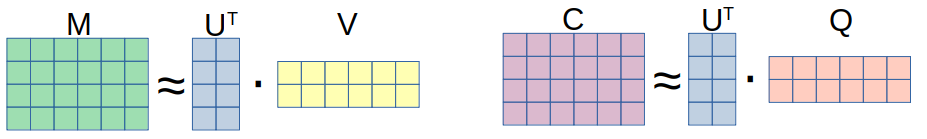
\includegraphics[width=0.8\linewidth]{images/mf2} \caption{Schematic representation of the proposed matrix co-factorization.}\label{fig:figshem}
\end{figure}

Because of the non-negativity of the entries in \(M\) and \(C\), it makes sense to restrict at least \(U\) to be non-negative. This enhances the interpretability of the resulting topics (Kuang, Choo, and Park (2015), Albalawi, Yeap, and Benyoucef (2020)). So the minimization is subject to:

\begin{equation}U, V,Q \geq 0 \text{ elementwise.}\label{eq:cons}
\end{equation}

The corresponding algorithm for minimizing \eqref{eq:minc} under the constraint \eqref{eq:cons} is based on the alternating minimization/ alternating projection in form of the hierarchical non-negative alternating least squares (HALS) of Cichocki, Zdunek, and Amari (2007) with our modification for the co-factorization setup (see also Degleris et al. (2019)).

For the loss function \(J(U,V,Q)\), we have:

\begin{align*}J(U,V,Q) &= ||M-U^\top V||^2 + \lambda ||C-U^\top Q|| \\
&= ||M-\sum_{k=1}^K u_kv_k^\top||^2 + \lambda ||C-\sum_{k=1}^K u_kq_k^\top||\\
&=||M-\sum_{k\not=p} u_kv_k^\top - u_pv_p^\top||^2 + \lambda ||C-\sum_{k\not=p} u_kq_k^\top - u_pq_p^\top||\\
&= Tr((M-\sum_{k\not=p} u_kv_k^\top)^\top (M-\sum_{k\not=p} u_kv_k^\top) - 2(M-\sum_{k\not=p} u_kv_k^\top)u_pv_p^\top + u_pv_p^\top v_p u_p) + \\
&+\lambda Tr((C-\sum_{k\not=p} u_kq_k^\top)^\top (C-\sum_{k\not=p} u_kq_k^\top) - 2(C-\sum_{k\not=p} u_kq_k^\top)u_pq_p^\top + u_pq_p^\top q_p u_p).
\end{align*}

The derivative with respect to \(u_p\) is:

\[\frac{\partial J(U,V,Q)}{\partial u_p} = - 2(M-\sum_{k\not=p} u_kv_k^\top)v_p^\top + 2u_pv_p^\top v_p - 2\lambda (C-\sum_{k\not=p} u_kq_k^\top)q_p^\top + 2\lambda u_pq_p^\top q_p.\]

Hence with Karush-Kuhn-Tucker conditions for optimality:

\[u_p = \max\left(0, \frac{(M-\sum_{k\not=p} u_kv_k^\top)v_p^\top + \lambda (C-\sum_{k\not=p} u_kq_k^\top)q_p^\top)}{v_p^\top v_p + \lambda q_p^\top q_p}\right).\]

The update rules for \(v_p\) and \(q_p\) do not differ from the HALS algorithm for NMF in Cichocki, Zdunek, and Amari (2007), that is:

\[v_p = \max\left(0, \frac{u_p(M-\sum_{k\not=p} u_kv_k^\top)}{u_p^\top u_p}\right),\]

\[q_p = \max\left(0, \frac{u_p(C-\sum_{k\not=p} u_kq_k^\top)}{u_p^\top u_p}\right).\]

The resulting Algorithm 1 is presented below.

\begin{algorithm}[H]
\begin{algorithmic}
\REQUIRE $K, \lambda$
\WHILE{not converged}
\FOR{$k=1$ to $K$}
\STATE update $V_k\leftarrow \max\left(\frac{U_k(M-U_{-k}^\top V_{-k})}{U_kU_k^\top },0\right)$
\STATE update $Q_k\leftarrow \max\left(\frac{U_k(C-U_{-k}^\top Q_{-k})}{U_kU_k^\top},0\right)$
\STATE update $U_k^\top \leftarrow \max\left(\frac{(M-U_{-k}^\top V_{-k})V_k^\top + \lambda (C-U_{-k}^\top Q_{-k})Q_k^\top}{ V_k^\top V_k  + \lambda Q_k^\top Q_k },0\right)$
\ENDFOR
\ENDWHILE
\end{algorithmic}
\caption{HALS algorithm for NMCF}
\end{algorithm}

\(X_k\) denotes the \(k\)th row of the matrix \(X\) and \(X_{-k}\) denotes the matrix without its \(k\)th row.

In summary, for a given \(K\) and \(\lambda\), the algorithm delivers a common low dimensional representation of \(M\) and \(C\) optimal in the sense of minimizing \(J(U,V,Q)\) under the non-negativity condition. \(U\) represents thereby a common latent topic space and \(V,Q\) are the low dimensional embeddings for the respective contexts in the topic space. The resulting low dimensional representation of corporate reports together with SDGs create a basis for choosing, evaluating and monitoring investments with respect to their impact on the society and the environment.

\hypertarget{application-of-nmcf}{%
\section{Application of NMCF}\label{application-of-nmcf}}

In this section, we apply the proposed algorithm to the bag-of-words representations of the reports and SDG texts. The associated NMCF algorithm requires the input of two nuisance parameter values. The first parameter \(\lambda\) governs the importance of the side information in the co-factorization procedure. The second parameter \(K\) specifies the number of latent topics and thus the resulting dimension of the latent topic space. We propose a data-driven procedure for the choice of \(K\) and \(\lambda\) based on maximizing the average topic coherence, present and visualize the resulting topic representations, and demonstrate their usefulness for sustainability assessment using cosine similarity.

\hypertarget{tuning-the-model}{%
\subsection{Tuning the model}\label{tuning-the-model}}

In order to accomplish the NMCF via the Algorithm 1, we have to specify the number of topics \(K\) (which corresponds to the dimension of the latent topic space) and the nuisance parameter \(\lambda\) for the loss function. Moreover, several weighting schemes for the term-context matrix are available. In this section, we test different weighting schemes and propose a data-driven procedure to simultaneously choose \(K\) and \(\lambda\) using their plausible ranges and maximizing topic coherence.

Coherence of topics is a popular metric for semantic validation of topic quality based on word co-occurrence (Thompson and Mimno (2018), Selivanov, Bickel, and Wang (2022)). According to Gurdiel, Morales Mediano, and Cifuentes Quintero (2021) coherence-based choice of topic number produces topics, interpretable for humans. Specifically, we employ the average mean-logratio topic coherence based on the internal text corpora of the reports and the SDGs.

The log coherence for a topic \(k\) with \(m\) top words \(w_{k,1},\ldots, w_{k,m}\), \(coh_k\), is given as:

\begin{equation}
coh_{k}=\sum_{i=1}^m\sum_{j<i}\log\frac{\#(w_{k,i},w_{k,j})}{\#(w_{k,i})}+\varepsilon,\label{eq:coh}
\end{equation}

where \(\#(\cdot)\) counts the contexts containing the input (a word or a word pair) and \(\varepsilon\) is a smoothing parameter. This metric quantifies how often the top \(m\) words in a topic \(k\) co-occur in the reference text corpus. It is justified by the observation that words with similar meaning tend to co-occur in the same contexts. That is, coherence of a topic is positively associated with its interpretability.

To find the optimal values for the nuisance parameters in the sense of maximum topic coherence, we create the meaningful combinations of \(K\) and \(\lambda\) with \(K=5,\ldots,15\) and \(\lambda\in[0,700],\) apply the NMCF algorithm to our data, and compute the log coherence for each topic as defined in \eqref{eq:coh}. We subsequently average the coherence measures over all topics:

\begin{equation}
\overline{coh}=\frac 1k \sum_{k=1}^Kcoh_k.\label{eq:acoh}
\end{equation}

As weighting alternatives, we use

\begin{itemize}
\tightlist
\item
  counts of term \(i\) in context \(j\), \(tf_{ij}\), (labelled as ``none''),
\item
  counts weighted by total frequency, \(tf_{ij}/\sum_{j}tf_{ij}\) (labelled as ``tf''),
\item
  counts weighted by total inverse frequency (labelled as ``tf-idf''),
\item
  logarithms of the counts, computed as \(1+\log_{10}(tf_{ij})\) for \(tf_{ij}>0\) and zero else (labelled as ``logcount''), and
\item
  logarithms of the counts standardized by average logcounts, computed as \(\frac{1+\log_{10}(tf_{ij})}{1+\log\left(\overline{tf_{ij}}\right)}\) (labelled as ``logave'').
\end{itemize}

For each weighting scheme above, we choose the combination of \(K\) and \(\lambda\) which results in the highest average log coherence computed by \eqref{eq:acoh}.
The resulting optimal parameter values , \(K\) and \(\lambda\), for different weighting schemes are shown in Table \ref{tab:tab00}. Finally, we choose the weighting and the combination of \(K\) and \(\lambda\) which result in the highest average log coherence.
Given the results in Table \ref{tab:tab00}, overall the tqo logarithmic weighting schemes seem to give the best results regarding the average coherence. The highest average coherence is obtained by using logarithmic counts in the term-context matrices, \(K=6\) topics, and \(\lambda=390.\) Thus, we use this parameter combination for our further analysis.

\begin{table}

\caption{\label{tab:tab00}The resulting optimal parameter values for different weighting schemes, $K$ and $\lambda$ using grid-search algorithm on maximum average coherence.}
\centering
\begin{tabular}[t]{l|l|l|l|l|l}
\hline
weighting & $\lambda$ & $K$ & $\overline{coh}$ (reports) & $\overline{coh}$ (SDGs) & $\overline{coh}$ (all)\\
\hline
none & 334 & 8 & -2.62348 & -0.94501 & -1.78425\\
\hline
tf & 660 & 8 & -2.25165 & -1.58800 & -1.91982\\
\hline
tf-idf & 346 & 15 & -6.09706 & -2.04164 & -4.06935\\
\hline
logcount & 390 & 6 & -2.40807 & -0.64715 & -1.52761\\
\hline
logave & 432 & 6 & -2.42982 & -0.64560 & -1.53771\\
\hline
\end{tabular}
\end{table}

\hypertarget{comparing-the-optimized-model-with-a-competing-technique-keyword-seeded-lda}{%
\subsection{Comparing the optimized model with a competing technique: keyword seeded LDA}\label{comparing-the-optimized-model-with-a-competing-technique-keyword-seeded-lda}}

In the following, we asses the performance of our model in comparison to a competitive technique: keyword seeded topic model (keyATM) introduced in Eshima, Imai, and Sasaki (n.d.). This technique is a state-of-the-art Bayesian method for extracting topics with a specific focus achieved by utilizing user-specified topic-specific keywords in the topic prior distributions. The requirement of the methodology is to supply user-specified topics with keywords. However, with the SDGs texts as side information, we do not have such topics with keywords at hand. Therefore, we employ the following two-stage procedure to obtain an analogy to our model:

\begin{itemize}
\tightlist
\item
  Obtain topic keywords by applying the classical LDA model to the SDG texts. The keywords are then a certain number of topwords for the extracted topics.
\item
  Plug-in the keywords in the keyATM to extract keyword assisted topics.
\end{itemize}

That is, in the first stage, we fit the classical LDA model based on the SDG texts only. We have to choose the number of topics for this model. Based on the average topic coherence, we choose the number of topics in a data-driven manner as in the previous section. According to our coherence criterion \eqref{eq:acoh}, the optimal topic number in this LDA model is \(K=6\). The top 10 words for each extracted topic constitute our keywords set for the next stage. The resulting keywords are summarized in Table \ref{tab:tabk}.

\begin{table}

\caption{\label{tab:tabk}The keywords (top 10 topic words) associated with the six topics extracted by LDA.}
\centering
\begin{tabular}[t]{l|l}
\hline
Category & Keywords\\
\hline
topic 1 & food, ecosystem, sourc, agricultur, land, protect, effici, natur, suppli, system\\
\hline
topic 2 & water, employ, innov, guidelin, work, overview, institut, labor, local, growth\\
\hline
topic 3 & sector, complet, benefit, inform, disclosur, consumpt, base, wast, least, solut\\
\hline
topic 4 & poverti, infrastructur, inclus, public, financ, measur, industri, overview, may, world\\
\hline
topic 5 & health, women, right, opportun, qualiti, compani, medicin, found, men, care\\
\hline
topic 6 & build, climat, resili, marin, afford, integr, ocean, plan, transport, solut\\
\hline
\end{tabular}
\end{table}

Besides the keyword topics, keyATM adopts a user-specified number of keywordless topics, which must also be provided. We use the top words for each LDA topic from the first stage and fit a keyword topic model with the six keyword topics and a varying number (zero to four) of additional topics without keywords. Subsequently, we compute the average coherence for the resulting models. The results are presented in Table \ref{tab:tabrcoh}. The best achieved average topic coherence is much lower than the one reported by our proposed model, demonstrating its advantage.

We should mention here, however, that we did not calibrate any parameters of the keyATM priors. Such calibration could potentially improve the results. Still, in this competitive approach, we have to calibrate both the first and second stage models to arrive at the resulting topic extraction with the embedded side information contained in the SDGs. Moreover, one has to consider the additional uncertainty brought by such a ``plug-in'' estimator. In contrast, with our proposed model, we calibrated the nuisance parameters just once and estimated the decomposition in a single stage.

\begin{table}

\caption{\label{tab:tabrcoh}The results on average coherence for the six keyword topics achieved by keyATM.}
\centering
\begin{tabular}[t]{l|l|l|l}
\hline
total number of topics & $\overline{coh}$ (all) & $\overline{coh}$ (reports) & $\overline{coh}$ (SDGs)\\
\hline
6 & -4.35951 & -1.20522 & -7.51379\\
\hline
7 & -4.17859 & -1.12814 & -6.86721\\
\hline
8 & -4.26095 & -1.10142 & -7.74990\\
\hline
9 & -4.24789 & -1.19756 & -7.21985\\
\hline
10 & -4.28675 & -1.14048 & -7.74389\\
\hline
\end{tabular}
\end{table}

\hypertarget{interpreting-the-best-nnmf-model}{%
\subsection{Interpreting the best NNMF model}\label{interpreting-the-best-nnmf-model}}

The output of Algorithm 1 are the decomposition matrices \(V,U\) and \(Q\). \(U\) contains the term-topic representations. By looking at the largest entries of \(U\) and the corresponding terms (the topwords), we can interpret the resulting latent topics. The entries of \(V,Q\) and their relative magnitudes reveal the proportions (or the importance) of the topics in the text corpus.

\begin{figure}
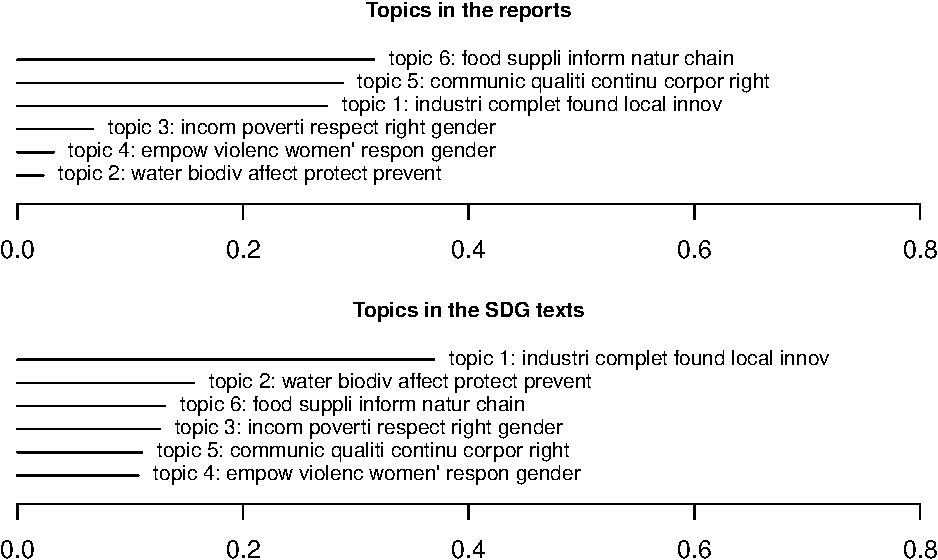
\includegraphics[width=0.8\linewidth]{20240606_sustain_dim_files/figure-latex/figtpropg-1} \caption{Topic proportion and the words with the highest weight per topic for each of the discovered topics in the reports (top) and in the SDG texts (bottom).}\label{fig:figtpropg}
\end{figure}

Figure \ref{fig:figtpropg} shows the topic proportions and the words with the highest weight per topic for each of the discovered topics in the reports and the SGD texts respectively. The top five words shown in Figure \ref{fig:figtpropg} already allow for satisfactory topic interpretation. The distribution of the topics is somewhat different in the reports compared to the SDG texts. The topic ``industri complet found local innov'' becomes a large share in the distribution of both the reports and the SDGs. Whereas the topics ``communic qualiti continu corpor right'' and ``water biodiv affect protect prevent'' seem to dominate the reports and the SDGs respectively. Clearly, using this kind of topic proportion representation allows for discovering new action areas for the companies.

In summary, the entries of \(V\) and \(Q\) deliver the \(k\)-dimensional context-topic representations enabling us to compare the underlying contexts in a low dimensional topic space using the embeddings of the contexts, which correspond to the entries of \(V\) and \(Q\).
Using the obtained representations of the corporate reports together with the SDGs in the following, we show a couple of strategies for choosing, evaluating and monitoring investments with respect to their impact on society and the environment in the next subsection.

\hypertarget{associating-the-reports-with-the-sdgs}{%
\subsection{Associating the reports with the SDGs}\label{associating-the-reports-with-the-sdgs}}

Now we employ a popular cosine similarity measure for text contents to associate the reports to the SDGs. Other (dis)similarity measures can be used based on our proposed topic embeddings with side information focus. Since cosine similarity tends to perform better than other dissimilarity measures in text comparison tasks (see i.e. Alobed, Altrad, and Bakar (2021)), the usage of cosine similarity in our association analysis is more inline with the main-stream text mining literature.

Since in our analysis each report is a combination of several contexts, each represented in a \(8\)-dimensional topic space, we need to aggregate the context-based similarity measures to a report level. We use the maximum for the aggregation over all contexts to the report level.

To obtain the resulting similarities, visualized in Figure \ref{fig:figcos}, we associate the report contents to the SDGs using the maximum cosine similarity. Therefore, we first compute the cosine similarity between each context of a report and each SDG, and then take the maximum over all report contexts as the resulting similarity measure.

\begin{figure}
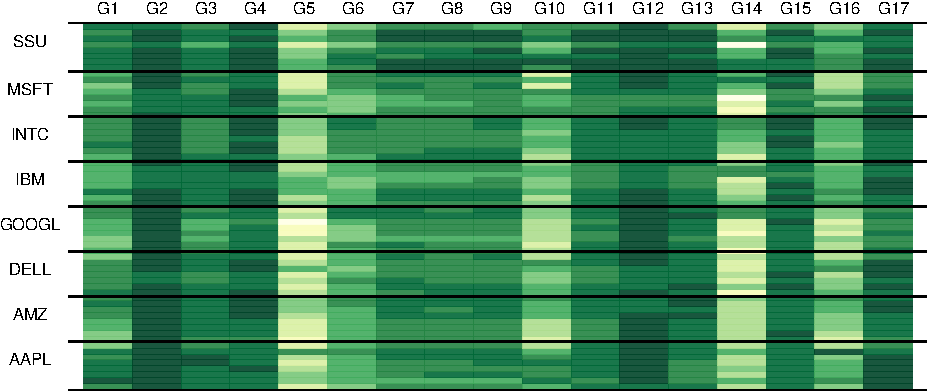
\includegraphics[width=1\linewidth]{20240606_sustain_dim_files/figure-latex/figcos-1} \caption{Similarity measures between the reports over the available company-years (rows, starting with earlier years on the bottom) and the SDGs (columns) computed using the resulting topic embeddings using maximum cosine similarity. Darker colors correspond to higher similarity values.}\label{fig:figcos}
\end{figure}

Note, that the similarity measures in Figure \ref{fig:figcos} are computed for each company-year enabling dynamic analysis of the underlying SDG related content and the associated progress in company sustainability actions evolution over time.

For a static analysis, we can use the \emph{average} the cosine similarities over the all available report years and construct a similarity-based rating of the considered firms with respect to each of the SDGs. The associated similarity-based rating is presented in Table \ref{tab:tab02}.

\begin{table}[H]
\centering
\caption{\label{tab:tab02}Company similarity-based rating (from the most similar to the least similar) with respect to the individual SDGs using the obtained topic embeddings pooled over all available report years.}
\centering
\begin{tabular}[t]{l|l}
\hline
Goal & Rating\\
\hline
G1 & SSU, AMZ, DELL, IBM, AAPL, INTC, MSFT, GOOGL\\
\hline
G2 & AAPL, AMZ, GOOGL, IBM, SSU, INTC, DELL, MSFT\\
\hline
G3 & AMZ, AAPL, SSU, IBM, MSFT, DELL, INTC, GOOGL\\
\hline
G4 & AMZ, INTC, IBM, SSU, MSFT, DELL, AAPL, GOOGL\\
\hline
G5 & SSU, INTC, IBM, AMZ, MSFT, DELL, AAPL, GOOGL\\
\hline
G6 & IBM, SSU, AMZ, INTC, DELL, AAPL, MSFT, GOOGL\\
\hline
G7 & SSU, AMZ, IBM, DELL, GOOGL, AAPL, MSFT, INTC\\
\hline
G8 & SSU, AMZ, IBM, AAPL, DELL, INTC, MSFT, GOOGL\\
\hline
G9 & SSU, AMZ, IBM, INTC, DELL, AAPL, MSFT, GOOGL\\
\hline
G10 & SSU, DELL, AMZ, AAPL, MSFT, INTC, IBM, GOOGL\\
\hline
G11 & SSU, AMZ, IBM, INTC, AAPL, MSFT, DELL, GOOGL\\
\hline
G12 & AAPL, IBM, SSU, GOOGL, AMZ, INTC, DELL, MSFT\\
\hline
G13 & AMZ, SSU, IBM, DELL, GOOGL, AAPL, INTC, MSFT\\
\hline
G14 & SSU, IBM, INTC, AAPL, MSFT, AMZ, DELL, GOOGL\\
\hline
G15 & IBM, INTC, AMZ, DELL, SSU, GOOGL, AAPL, MSFT\\
\hline
G16 & SSU, IBM, AMZ, INTC, MSFT, DELL, AAPL, GOOGL\\
\hline
G17 & DELL, AMZ, SSU, INTC, AAPL, IBM, MSFT, GOOGL\\
\hline
\end{tabular}
\end{table}

In our framework, we are not restricted to associating the reports to the individual SDGs only. We are also able to consider any linear combinations of the goals composed based on personal preferences, such that, in a sense, a personalized sustainability goal for a tailored sustainability assessment can be easily created. In order to considering individual preferences, let us define a linear combination of the goals using weights \(\beta=(\beta_1,\ldots,\beta_{17})^\top\). Then \(C\beta\approx UQ^\top\beta\) defines a ``personalized'' goal based on the term occurrences approximated by the co-factorization. Using the following four different combinations (portfolios) of SDGs, we provide an example of such tailored sustainability assessment.

Our example portfolios are:

\begin{itemize}
\tightlist
\item
  ``all\_equal'' (all goals are equally weighted),
\item
  ``basic\_needs'' (the goals addressing the basic human needs (SDGs 1-6) are equally weighted and all other goals have zero weights),
\item
  ``fair\_society'' (the goals concerning society and infrastructure developement (SDGs 7-12 and 16-17) are equaly weighted and all other goals have zero weights),
\item
  ``climate\_life'' (the goals addressing climate, plant and animal life (SDGs 13-15) are equally weighted and all other goals have zero weights).
\end{itemize}

\begin{table}

\caption{\label{tab:tab03}Company similarity-based rating (from the most similar to the least similar) with respect to the individual SDGs using the obtained topic embeddings for the reports in year 2020 .}
\centering
\begin{tabular}[t]{l|l}
\hline
goal & rating\\
\hline
all\_equal & SSU, INTC, MSFT, AMZ, IBM, AAPL, DELL, GOOGL\\
\hline
basic\_needs & AMZ, INTC, SSU, MSFT, IBM, DELL, AAPL, GOOGL\\
\hline
fair\_society & INTC, MSFT, SSU, IBM, AAPL, AMZ, DELL, GOOGL\\
\hline
climate\_life & SSU, INTC, AMZ, AAPL, MSFT, IBM, GOOGL, DELL\\
\hline
\end{tabular}
\end{table}

In Table \ref{tab:tab03}, the resulting firm rating based on each SDG portfolio is presented. As shown, the ratings can be quite different depending on the concrete preferences. In general, any linear combination of the goals can build a basis for such a comparison. This makes the proposed procedure very flexible. Moreover, any user defined (dis)similarity metric can be applied to the resulting embeddings in the topic space, which grant additional flexibility to our method.

In summary, as shown in the above analysis, the proposed matrix co-factorization for sustainability assessment with respect to the predefined structure of the 17 SDGs, is a transparent and flexible approach resulting in a low dimensional topic representation facilitating adaptive association of the sustainability related reports with the SDGs.

\hypertarget{conclusion-and-discussion}{%
\section{Conclusion and Discussion}\label{conclusion-and-discussion}}

In the present paper, we propose a transparent approach that enables us to represent the textual content of sustainanbility reports in a topic space using the 17 SDGs as a predefined structure. The proposed methodology builds upon non-negative matrix co-factorization for topic extraction with side information, resulting in a low-dimensional representation in a prestructured topic space. The method is scalable, simple to implement, computationally efficient, and does not require any manual intervention as other comparable methods do. It delivers transparent and interpretable results with many use cases.

The adopted matrix co-factorization jointly factorizes two term-context matrices: the first one contains the term-context counts for the corpus of sustainability-related reports, and the second one contains the term-context counts for the SDG texts, representing the predefined structure or the side information. The associated algorithm, based on hierarchical NMF, requires the input of two nuisance parameter values. The first nuisance parameter, \(\lambda\), governs the importance of the side information in the co-factorization procedure. The second nuisance parameter, \(K\), specifies the number of latent topics and thus the resulting dimension of the latent topic space. We test multiple weighting schemes for the term-context representations and provide a data-driven procedure for choosing the values of the nuisance parameters by maximizing the common goodness-of-fit measure for unsupervised topic extraction: the average topic coherence.

Using average topic coherence as the goodness-of-fit criterion, we compare our proposed method to a comparable competing technique - keyword seeded topic model from Eshima, Imai, and Sasaki (n.d.). The results show that our model outperforms the competitor in terms of the average topic coherence and represents a computationally simpler method to achieve directed topic extraction.

Our results in form of directed contextual topic embeddings provide a basis for dynamic comparison of the sustainability-related reports for eight listed tech firms. We associate the reports with the SDGs using maximum cosine similarity and show that our procedure can efficiently assist financial decisions under tailored SDG-based preferences.

Nevertheless, an important premise of our analysis is that the reports' texts contain objective information on firms' sustainability actions, which may not hold in general. Laskin and Nesova (2022) discuss the issue of the credibility of sustainability reports and point out a bias towards optimistic language. Moreover, we do not take into consideration the sentiment associated with the report content (positive or negative tone), which is an important aspect of sustainability assessment (Mućko (2021)). Incorporating these issues into the analysis is a promising subject for future research.

\hypertarget{references}{%
\section*{References}\label{references}}
\addcontentsline{toc}{section}{References}

\begin{verbatim}
## character(0)
\end{verbatim}

\hypertarget{refs}{}
\begin{CSLReferences}{1}{0}
\leavevmode\vadjust pre{\hypertarget{ref-albalawi2020}{}}%
Albalawi, Rania, Tet Hin Yeap, and Morad Benyoucef. 2020. {``Using Topic Modeling Methods for Short-Text Data: A Comparative Analysis.''} \emph{Frontiers in Artificial Intelligence} 3. \url{https://doi.org/10.3389/frai.2020.00042}.

\leavevmode\vadjust pre{\hypertarget{ref-alobed2021}{}}%
Alobed, Mohammad, Abdallah M M Altrad, and Zainab Binti Abu Bakar. 2021. {``A Comparative Analysis of Euclidean, Jaccard and Cosine Similarity Measure and Arabic Wordnet for Automated Arabic Essay Scoring.''} In \emph{2021 Fifth International Conference on Information Retrieval and Knowledge Management (CAMP)}, 70--74. \url{https://doi.org/10.1109/CAMP51653.2021.9498119}.

\leavevmode\vadjust pre{\hypertarget{ref-amini2018}{}}%
Amini, Mehdi, Carol C. Bienstock, and John A. Narcum. 2018. {``Status of Corporate Sustainability: A Content Analysis of Fortune 500 Companies.''} \emph{Business Strategy and the Environment} 27 (8): 1450--61. https://doi.org/\url{https://doi.org/10.1002/bse.2195}.

\leavevmode\vadjust pre{\hypertarget{ref-quanteda}{}}%
Benoit, Kenneth, Kohei Watanabe, Haiyan Wang, Paul Nulty, Adam Obeng, Stefan Müller, and Akitaka Matsuo. 2018. {``Quanteda: An r Package for the Quantitative Analysis of Textual Data.''} \emph{Journal of Open Source Software} 3 (30): 774. \url{https://doi.org/10.21105/joss.00774}.

\leavevmode\vadjust pre{\hypertarget{ref-berg2022}{}}%
Berg, Florian, Julian F Kölbel, and Roberto Rigobon. 2022. {``{Aggregate Confusion: The Divergence of ESG Ratings*}.''} \emph{Review of Finance} 26 (6): 1315--44. \url{https://doi.org/10.1093/rof/rfac033}.

\leavevmode\vadjust pre{\hypertarget{ref-blei2003}{}}%
Blei, David M., Andrew Y. Ng, and Michael I. Jordan. 2003. {``Latent Dirichlet Allocation.''} \emph{J. Mach. Learn. Res.} 3 (null): 993--1022.

\leavevmode\vadjust pre{\hypertarget{ref-chen2023}{}}%
Chen, Weisi, Fethi Rabhi, Wenqi Liao, and Islam Al-Qudah. 2023. {``Leveraging State-of-the-Art Topic Modeling for News Impact Analysis on Financial Markets: A Comparative Study.''} \emph{Electronics} 12 (12). \url{https://doi.org/10.3390/electronics12122605}.

\leavevmode\vadjust pre{\hypertarget{ref-CHEN2019}{}}%
Chen, Yong, Hui Zhang, Rui Liu, Zhiwen Ye, and Jianying Lin. 2019. {``Experimental Explorations on Short Text Topic Mining Between LDA and NMF Based Schemes.''} \emph{Knowledge-Based Systems} 163: 1--13. https://doi.org/\url{https://doi.org/10.1016/j.knosys.2018.08.011}.

\leavevmode\vadjust pre{\hypertarget{ref-chen2017}{}}%
Chen, Yu, Rhaad M. Rabbani, Aparna Gupta, and Mohammed J. Zaki. 2017. {``Comparative Text Analytics via Topic Modeling in Banking.''} In \emph{2017 IEEE Symposium Series on Computational Intelligence (SSCI)}, 1--8. \url{https://doi.org/10.1109/SSCI.2017.8280945}.

\leavevmode\vadjust pre{\hypertarget{ref-churchill2022}{}}%
Churchill, Rob, and Lisa Singh. 2022. {``The Evolution of Topic Modeling.''} \emph{ACM Comput. Surv.} 54 (10s). \url{https://doi.org/10.1145/3507900}.

\leavevmode\vadjust pre{\hypertarget{ref-cichocki2007}{}}%
Cichocki, Andrzej, Rafal Zdunek, and Shun-ichi Amari. 2007. {``Hierarchical ALS Algorithms for Nonnegative Matrix and 3D Tensor Factorization.''} In \emph{Independent Component Analysis and Signal Separation}, edited by Mike E. Davies, Christopher J. James, Samer A. Abdallah, and Mark D. Plumbley, 169--76. Berlin, Heidelberg: Springer Berlin Heidelberg.

\leavevmode\vadjust pre{\hypertarget{ref-deerwester1990}{}}%
Deerwester, Scott, Susan T. Dumais, George W. Furnas, Thomas K. Landauer, and Richard Harshman. 1990. {``Indexing by Latent Semantic Analysis.''} \emph{Journal of the American Society for Information Science} 41 (6): 391--407. https://doi.org/\url{https://doi.org/10.1002/(SICI)1097-4571(199009)41:6\%3C391::AID-ASI1\%3E3.0.CO;2-9}.

\leavevmode\vadjust pre{\hypertarget{ref-degleris2019}{}}%
Degleris, Anthony, Ben Antin, Surya Ganguli, and Alex H Williams. 2019. {``Fast Convolutive Nonnegative Matrix Factorization Through Coordinate and Block Coordinate Updates.''} \url{https://arxiv.org/abs/1907.00139}.

\leavevmode\vadjust pre{\hypertarget{ref-egger2022}{}}%
Egger, Roman, and Joanne Yu. 2022. {``A Topic Modeling Comparison Between LDA, NMF, Top2Vec, and BERTopic to Demystify Twitter Posts.''} \emph{Frontiers in Sociology} 7. \url{https://doi.org/10.3389/fsoc.2022.886498}.

\leavevmode\vadjust pre{\hypertarget{ref-eshima2023}{}}%
Eshima, Shusei, Kosuke Imai, and Tomoya Sasaki. n.d. {``Keyword-Assisted Topic Models.''} \emph{American Journal of Political Science} n/a (n/a). https://doi.org/\url{https://doi.org/10.1111/ajps.12779}.

\leavevmode\vadjust pre{\hypertarget{ref-fang2011}{}}%
Fang, Yi, and Luo Si. 2011. {``Matrix Co-Factorization for Recommendation with Rich Side Information and Implicit Feedback.''} In \emph{Proceedings of the 2nd International Workshop on Information Heterogeneity and Fusion in Recommender Systems}, 65--69. HetRec '11. New York, NY, USA: Association for Computing Machinery. \url{https://doi.org/10.1145/2039320.2039330}.

\leavevmode\vadjust pre{\hypertarget{ref-figuera2024}{}}%
Figuera, Pau, and Pablo García Bringas. 2024. {``Revisiting Probabilistic Latent Semantic Analysis: Extensions, Challenges and Insights.''} \emph{Technologies} 12 (1). \url{https://doi.org/10.3390/technologies12010005}.

\leavevmode\vadjust pre{\hypertarget{ref-gupta2020}{}}%
Gupta, Aaryan, Vinya Dengre, Hamza Abubakar Kheruwala, and Manan Shah. 2020. {``Comprehensive Review of Text-Mining Applications in Finance.''} \emph{Financial Innovation} 6 (1): 1--25. \url{https://doi.org/10.1186/s40854-020-00205-1}.

\leavevmode\vadjust pre{\hypertarget{ref-gurdiel2021}{}}%
Gurdiel, Lidia, Javier Morales Mediano, and Jenny Cifuentes Quintero. 2021. {``A Comparison Study Between Coherence and Perplexity for Determining the Number of Topics in Practitioners Interviews Analysis.''} In.

\leavevmode\vadjust pre{\hypertarget{ref-Harandizadeh2022}{}}%
Harandizadeh, Bahareh, J. Hunter Priniski, and Fred Morstatter. 2022. {``Keyword Assisted Embedded Topic Model.''} In \emph{Proceedings of the Fifteenth {ACM} International Conference on Web Search and Data Mining}. {ACM}. \url{https://doi.org/10.1145/3488560.3498518}.

\leavevmode\vadjust pre{\hypertarget{ref-hofmann1999}{}}%
Hofmann, Thomas. 1999. {``Probabilistic Latent Semantic Indexing.''} In \emph{Proceedings of the 22nd Annual International ACM SIGIR Conference on Research and Development in Information Retrieval}, 50--57. SIGIR '99. New York, NY, USA: Association for Computing Machinery. \url{https://doi.org/10.1145/312624.312649}.

\leavevmode\vadjust pre{\hypertarget{ref-kang2022}{}}%
Kang, Hyewon, and Jinho Kim. 2022. {``Analyzing and Visualizing Text Information in Corporate Sustainability Reports Using Natural Language Processing Methods.''} \emph{Applied Sciences} 12 (11). \url{https://doi.org/10.3390/app12115614}.

\leavevmode\vadjust pre{\hypertarget{ref-Kuang2015}{}}%
Kuang, Da, Jaegul Choo, and Haesun Park. 2015. {``Nonnegative Matrix Factorization for Interactive Topic Modeling and Document Clustering.''} In \emph{Partitional Clustering Algorithms}, edited by M. Emre Celebi, 215--43. Cham: Springer International Publishing. \url{https://doi.org/10.1007/978-3-319-09259-1_7}.

\leavevmode\vadjust pre{\hypertarget{ref-landrum2018}{}}%
Landrum, Nancy, and Brian Ohsowski. 2017. {``Identifying Worldviews on Corporate Sustainability: A Content Analysis of Corporate Sustainability Reports.''} \emph{Business Strategy and the Environment} 27 (November). \url{https://doi.org/10.1002/bse.1989}.

\leavevmode\vadjust pre{\hypertarget{ref-laskin2022}{}}%
Laskin, Alexander V., and Natalya Mikhailovna Nesova. 2022. {``The Language of Optimism in Corporate Sustainability Reports: A Computerized Content Analysis.''} \emph{Business and Professional Communication Quarterly} 85 (1): 80--98. \url{https://doi.org/10.1177/23294906211065507}.

\leavevmode\vadjust pre{\hypertarget{ref-lee2000}{}}%
Lee, Daniel, and H. Sebastian Seung. 2000. {``Algorithms for Non-Negative Matrix Factorization.''} In \emph{Advances in Neural Information Processing Systems}, edited by T. Leen, T. Dietterich, and V. Tresp. Vol. 13. MIT Press. \url{https://proceedings.neurips.cc/paper_files/paper/2000/file/f9d1152547c0bde01830b7e8bd60024c-Paper.pdf}.

\leavevmode\vadjust pre{\hypertarget{ref-LI2017}{}}%
Li, Guowen, Xiaoqian Zhu, Jun Wang, Dengsheng Wu, and Jianping Li. 2017. {``Using LDA Model to Quantify and Visualize Textual Financial Stability Report.''} \emph{Procedia Computer Science} 122: 370--76. https://doi.org/\url{https://doi.org/10.1016/j.procs.2017.11.382}.

\leavevmode\vadjust pre{\hypertarget{ref-LIEW2014}{}}%
Liew, Wan Te, Arief Adhitya, and Rajagopalan Srinivasan. 2014. {``Sustainability Trends in the Process Industries: A Text Mining-Based Analysis.''} \emph{Computers in Industry} 65 (3): 393--400. https://doi.org/\url{https://doi.org/10.1016/j.compind.2014.01.004}.

\leavevmode\vadjust pre{\hypertarget{ref-loughran2016}{}}%
Loughran, Tim, and Bill McDonald. 2016. {``Textual Analysis in Accounting and Finance: A Survey.''} \emph{Journal of Accounting Research} 54 (4): 1187--1230. https://doi.org/\url{https://doi.org/10.1111/1475-679X.12123}.

\leavevmode\vadjust pre{\hypertarget{ref-luo2019}{}}%
Luo, Ling, Haoran Xie, Yanghui Rao, and Fu Lee Wang. 2019. {``Personalized Recommendation by Matrix Co-Factorization with Tags and Time Information.''} \emph{Expert Systems with Applications} 119: 311--21. https://doi.org/\url{https://doi.org/10.1016/j.eswa.2018.11.003}.

\leavevmode\vadjust pre{\hypertarget{ref-MUCKO2021}{}}%
Mućko, Przemysław. 2021. {``Sentiment Analysis of CSR Disclosures in Annual Reports of EU Companies.''} \emph{Procedia Computer Science} 192: 3351--59. https://doi.org/\url{https://doi.org/10.1016/j.procs.2021.09.108}.

\leavevmode\vadjust pre{\hypertarget{ref-NUGUMANOVA2022}{}}%
Nugumanova, Aliya, Darkhan Akhmed-Zaki, Madina Mansurova, Yerzhan Baiburin, and Almasbek Maulit. 2022. {``NMF-Based Approach to Automatic Term Extraction.''} \emph{Expert Systems with Applications} 199: 117179. https://doi.org/\url{https://doi.org/10.1016/j.eswa.2022.117179}.

\leavevmode\vadjust pre{\hypertarget{ref-rr}{}}%
R Core Team. 2023. \emph{R: A Language and Environment for Statistical Computing}. Vienna, Austria: R Foundation for Statistical Computing. \url{https://www.R-project.org/}.

\leavevmode\vadjust pre{\hypertarget{ref-rao2015}{}}%
Rao, Nikhil, Hsiang-Fu Yu, Pradeep K Ravikumar, and Inderjit S Dhillon. 2015. {``Collaborative Filtering with Graph Information: Consistency and Scalable Methods.''} In \emph{Advances in Neural Information Processing Systems}, edited by C. Cortes, N. Lawrence, D. Lee, M. Sugiyama, and R. Garnett. Vol. 28. Curran Associates, Inc. \url{https://proceedings.neurips.cc/paper_files/paper/2015/file/f4573fc71c731d5c362f0d7860945b88-Paper.pdf}.

\leavevmode\vadjust pre{\hypertarget{ref-text2vec}{}}%
Selivanov, Dmitriy, Manuel Bickel, and Qing Wang. 2022. \emph{Text2vec: Modern Text Mining Framework for r}. \url{https://CRAN.R-project.org/package=text2vec}.

\leavevmode\vadjust pre{\hypertarget{ref-soh2014}{}}%
Soh, Dominic S. B. 2014. {``Sustainability Reporting and Assurance: A Historical Analysis on a World-Wide Phenomenon.''} \emph{Social and Environmental Accountability Journal} 34 (2): 125--25. \url{https://doi.org/10.1080/0969160X.2014.938484}.

\leavevmode\vadjust pre{\hypertarget{ref-SULEMAN2021}{}}%
Suleman, Raja Muhammad, and Ioannis Korkontzelos. 2021. {``Extending Latent Semantic Analysis to Manage Its Syntactic Blindness.''} \emph{Expert Systems with Applications} 165: 114130. https://doi.org/\url{https://doi.org/10.1016/j.eswa.2020.114130}.

\leavevmode\vadjust pre{\hypertarget{ref-thompson-mimno-2018}{}}%
Thompson, Laure, and David Mimno. 2018. {``Authorless Topic Models: Biasing Models Away from Known Structure.''} In \emph{Proceedings of the 27th International Conference on Computational Linguistics}, edited by Emily M. Bender, Leon Derczynski, and Pierre Isabelle, 3903--14. Santa Fe, New Mexico, USA: Association for Computational Linguistics. \url{https://aclanthology.org/C18-1329}.

\leavevmode\vadjust pre{\hypertarget{ref-tsalis2020}{}}%
Tsalis, Thomas A., Kyveli E. Malamateniou, Dimitrios Koulouriotis, and Ioannis E. Nikolaou. 2020. {``New Challenges for Corporate Sustainability Reporting: United Nations' 2030 Agenda for Sustainable Development and the Sustainable Development Goals.''} \emph{Corporate Social Responsibility and Environmental Management} 27 (4): 1617--29. https://doi.org/\url{https://doi.org/10.1002/csr.1910}.

\leavevmode\vadjust pre{\hypertarget{ref-vangara2020}{}}%
Vangara, Raviteja, Erik Skau, Gopinath Chennupati, Hristo Djidjev, Thomas Tierney, James P. Smith, Manish Bhattarai, Valentin G. Stanev, and Boian S. Alexandrov. 2020. {``Semantic Nonnegative Matrix Factorization with Automatic Model Determination for Topic Modeling.''} In \emph{2020 19th IEEE International Conference on Machine Learning and Applications (ICMLA)}, 328--35. \url{https://doi.org/10.1109/ICMLA51294.2020.00060}.

\leavevmode\vadjust pre{\hypertarget{ref-watanabe2022}{}}%
Watanabe, Kohei, and Yuan Zhou. 2022. {``Theory-Driven Analysis of Large Corpora: Semisupervised Topic Classification of the UN Speeches.''} \emph{Social Science Computer Review} 40 (2): 346--66. \url{https://doi.org/10.1177/0894439320907027}.

\leavevmode\vadjust pre{\hypertarget{ref-Yang2015}{}}%
Yang, Qingquan, and Weijiang Li. 2015/07. {``The LDA Topic Model Extension Study.''} In \emph{Proceedings of the International Conference on Logistics, Engineering, Management and Computer Science}, 857--60. Atlantis Press. \url{https://doi.org/10.2991/lemcs-15.2015.169}.

\leavevmode\vadjust pre{\hypertarget{ref-zahng2020_graph}{}}%
Zhang, Yupei, Yue Yun, Huan Dai, Jiaqi Cui, and Xuequn Shang. 2020. {``Graphs Regularized Robust Matrix Factorization and Its Application on Student Grade Prediction.''} \emph{Applied Sciences} 10 (5). \url{https://doi.org/10.3390/app10051755}.

\leavevmode\vadjust pre{\hypertarget{ref-Zhao2021}{}}%
Zhao, He, Dinh Q. Phung, Viet Huynh, Yuan Jin, Lan Du, and Wray L. Buntine. 2021. {``Topic Modelling Meets Deep Neural Networks: A Survey.''} In \emph{International Joint Conference on Artificial Intelligence}. \url{https://api.semanticscholar.org/CorpusID:232076325}.

\end{CSLReferences}

\end{document}
